\hyphenation{naj-po-pu-lar-niej-szym}
\chapter{Wstęp}
\label{sec:wstep}
\section{Wprowadzenie}
Sztuczna inteligencja to dziedzina wywodząca się z informatyki. Jej początki sięgają lat pięćdziesiątych XX wieku. Jeden z pierwszych badaczy,  John McCarthy, określił sztuczną inteligencję jako ,,naukę i technikę tworzącą inteligentne maszyny''. Pomimo zmian, jakie dokonały się w przeciągu kolejnych 60 lat, definicję tę wciąż można uznać za aktualną. Sztuczna inteligencja obejmuje kilka zagadnień, między innymi logikę rozmytą, sieci neuronowe czy planowanie \cite{ai}.

Automatyczne planowanie jest dziedziną sztucznej inteligencji, która zajmuje się realizacją sekwencji akcji oraz strategii \cite{planning}. Innymi słowy, zadaniem automatycznego planowania jest takie pokierwanie akcjami, by ze stanu początkowego dotrzeć do określonego stanu końcowego (celu). Najczęściej wymagany jest również jak najmniejszy czas lub koszt wykonania ułożonego planu. Istnieje kilka powszechnie znanych języków formalnych, umożliwiających wyrażanie problemu automatycznego planowania. Najbardziej znane języki to STRIPS (\textit{Stanford Research Institute Problem Solver}) \cite{strips} oraz PDDL (\textit{Planning Domain Definition Language}) \cite{pddl}, na którym opiera się projekt będący przedmiotem niniejszej pracy.
	
Język PDDL jest jednym z wyspecjalizowanych języków służących do opisu zagadnień związanych z automatycznym planowaniem. Został utworzony z przeznaczeniem na międzynarodowy konkurs planistyczny (IPC - \emph{International Planning Competition \footnote{http://ipc.icaps-conference.org/}}), mający miejsce w 1998 roku. Wzorowany był na innych językach wyspecjalizowanych w automatycznym planowaniu, między innymi na STRIPS'ie. W niektórych częściach języka PDDL można dostrzec podobieństwo do jego wzorca (na przykład w definiowanych akcjach), jednakże posiada on odmienną składnię.   

W celu wydajnego tworzenia oprogramowania, programiści korzystają z rozmaitych narzędzi. Zdarza się jednak, że samo ich wyszukiwanie i instalacja w systemie operacyjnym, zajmuje więcej czasu niż stworzenie programu. Rozwiązaniem są środowiska programistyczne, zapewniające w większości przypadków podstawowe funkcjonalności, oraz możliwość łatwego wyszukiwania i komponowania potrzebnych narzędzi.

\section{Motywacja}
Pomimo stworzenia PDDL, problemem jest znalezienie odpowiedniego, w pełni funkcjonalnego narzędzia. Obecnie dostępne rozwiązania posiadają istotne wady. Są to między innymi brak możliwości pracy z innym systemem  niż Windows, brakiem odpowiedniego formatowania kodu czy nieodpowiednim kolorowaniem składni. Założeniem projektu GUI4PDDL jest rozwiązanie większości niedogodności związanych z pisaniem programów w języku PDDL.

Obecnie istnieją środowiska programistyczne dla wielu języków. Na rysunku \ref{fig:srodowiskoprogramistyczne} przedstawiono środowisko \emph{Code::Blocks}\footnote{http://www.codeblocks.org/}, które jest 
jednym z narzędzi wspomagających programowanie w języku C++.

\begin{figure}[h!]
    \centering
    
    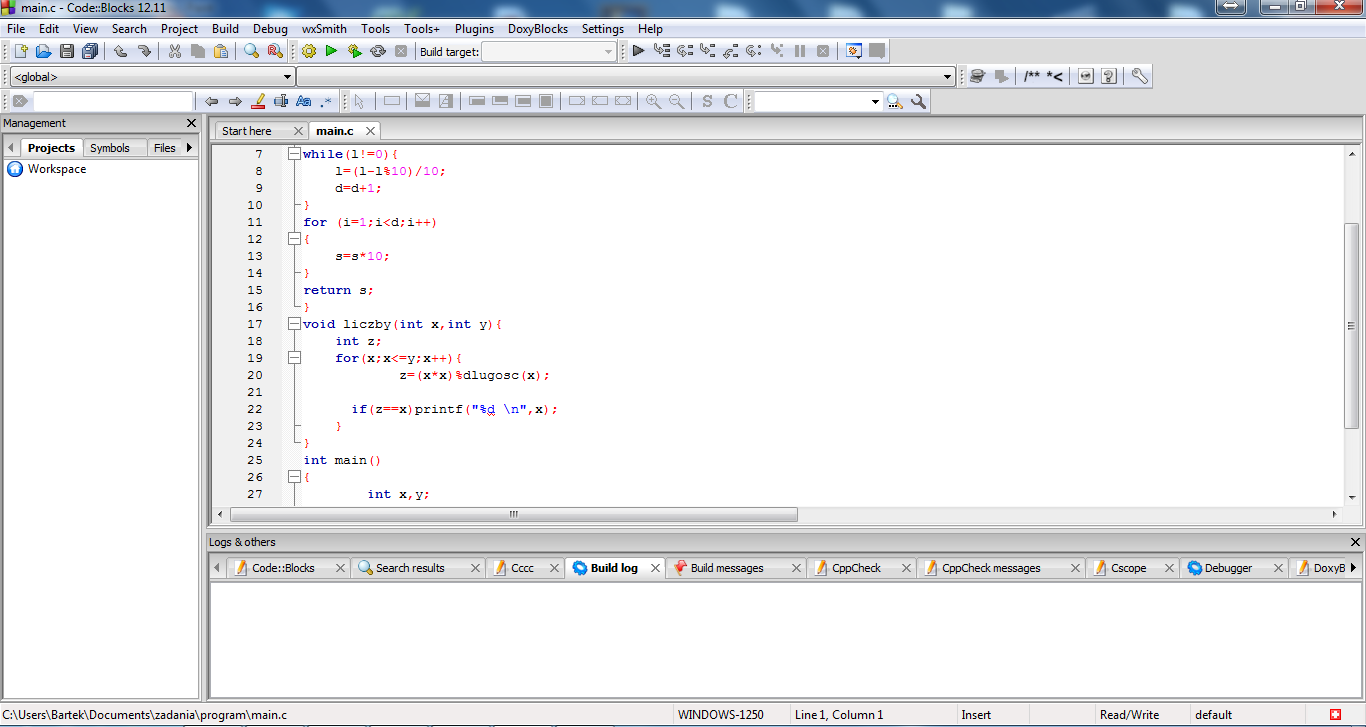
\includegraphics[width=\textwidth]{img/codeblocks}
    \caption{Przykładowe środowisko programistyczne}
    \label{fig:srodowiskoprogramistyczne}
\end{figure}

\section{Cel i zakres pracy}
Celem pracy jest stworzenie graficznego środowiska programistycznego, umożliwiającego pisanie programów w języku PDDL. Środowisko to powinno dostarczać przede wszystkim edytor kodu, zapewniający tworzenie automatycznych wcięć i kolorowanie składni, co pozwala zwiększyć przejrzystość struktury programu. Znaczącymi założeniami edytora są także podpowiadanie składni oraz wykrywanie błędów w kodzie źródłowym, które przyspieszają proces przygotowywania projektu. Dodatkowo, w~związku z wykorzystaniem dużej liczby nawiasów w PDDL, wymagane jest ich dopasowywanie. Dostępna powinna być również możliwość uruchamiania zewnętrznego oprogramowania do wyznaczania planu i przeglądania wyników planowania oraz zarządzania projektami i plikami.  

W pierwszej części drugiego rozdziału (roz \ref{sec:opis}), przedstawiona została problematyka automatycznego planowania. W rozdziale~\ref{sec:jezykpddl} opisany jest język PDDL, a następnie (roz.~\ref{sec:oprogramowanie}) opisano najważniejsze narzędzia służące do przeprowadzania procesu planowania.

Kolejny rozdział (roz. \ref{sec:specyfikacja}) to opis wymagań funkcjonalnych oraz wymagań pozafunkcjonalnych.

Rozdział czwarty podzielony jest na dwie części. W pierwszej z nich (roz. \ref{sec:eclipseśrodowisko})  opisane jest środowisko programistyczne Eclipse, w którym stworzona została wtyczka GUI4PDDL. Jest to również środowisko, na którym docelowo ma działać stworzony projekt. W drugiej części (roz. \ref{sec:antlrśrodowisko}) opisany został generator analizatorów składniowych ANTLR.

W rozdziale \ref{sec:piaty} przedstawiono architekturę tworzonego systemu, uwzględniając jego podział na projekty platformy \emph{Eclipse}. Opisana jest tu również szczegółowa zawartość każdego pakietu głównego projektu.

Następny rozdział (roz. \ref{sec:implementacja}) zawiera szczegółowe przedstawienie implementacji najważniejszych funkcjonalności. Opisane są tu kwestie tworzenia nowego projektu PDDL oraz nowych plików PDDL (roz. \ref{sec:zarzadzanie}).W kolejnej części ukazano zagadnienia związane z~przetwarzaniem kodu PDDL, czyli wykrywanie błędów składniowych i semantycznych oraz podpowiadanie kodu (roz. \ref{sec:przetwarzanie}). Dalej przedstawione są: kolorowanie kodu, automatyczne wcięcia, dopasowanie nawiasów oraz kwestie związane z obsługą podpowiedzi (roz. \ref{sec:edytor}).  Na końcu omówiono współpracę wtyczki z oprogramowaniem wyznaczającym plan, jego konfigurację i uruchamianie, a także przerywanie procesu planowania (roz. \ref{sec:wspolpraca}).

W rozdziale \ref{sec:testy} opisane są testy jednostkowe kodu oraz gramatyk formalnych. Dodatkowo przedstawiono testy akceptacyjne.

W ostatnim rozdziale \ref{sec:podsumowanie} zawarte jest podsumowanie pracy. W dodatku A opisana jest zawartość płyty CD dołączonej do pracy. Na końcu zawarta została bibliografia.
\section{Podział zadań}
W niniejszym podrozdziale zawarty jest zadań, wykonanych przez poszczególne osoby z grupy.\\\\
\begin{description}
  \item[Tomasz Boczkowski] \hfill 
  \begin{itemize}
\item Moduł analizy kodu PDDL
\item Wykrywanie błędów składniowych i semantycznych
\item Podpowiadanie składni
\item Praca pisemna, rozdziały: \ref{sec:antlrśrodowisko}, \ref{sec:przetwarzanie}, \ref{sec:podsumowanie}
\end{itemize}
  \item[Mateusz Michalak] \hfill 
    \begin{itemize}
\item Testy jednostkowe i integracyjne tworzonego oprogramowania
\item Witryna internetowa
\item Praca pisemna, rozdziały: \ref{sec:wstep}, \ref{sec:drugi}, \ref{sec:testy}
\end{itemize}
  \item[Wojciech Rybicki] \hfill 
    \begin{itemize}
\item Integracja wtyczki z istniejącymi narzędziami automatycznego planowania
\item Moduł do przeglądania danych wyjściowych
\item Praca pisemna, rozdziały: \ref{sec:piaty}, \ref{sec:wspolpraca}
\end{itemize}
  \item[Andrzej Płuszka] \hfill 
    \begin{itemize}
\item Edytor kodu PDDL i jego integracja z środowiskeim \textit{Eclipse}
\item Kolorowanie i podpowiadanie składni
\item Praca pisemna, rozdziały: \ref{sec:specyfikacja}, \ref{sec:eclipseśrodowisko}, \ref{sec:zarzadzanie}, \ref{sec:edytor}
\end{itemize}
\end{description}




